\documentclass{report}

\begin{document}

% 封面
\makecover{軟性計算}{Homework \#02\\[0.5em] PSO 訓練類神經網路}{S11159005}{黃毓峰}

\tableofcontents
\newpage

%=============================================================================
\section{開發環境}
%=============================================================================

\begin{table}[H]
\centering
\begin{tabular}{ll}
\toprule
\textbf{項目} & \textbf{版本} \\
\midrule
程式語言 & Rust 1.83.0 \\
編譯器 & rustc 1.83.0 (90b35a623 2024-11-26) \\
建構工具 & Cargo 1.83.0 \\
作業系統 & macOS 15.2 (Darwin 25.2.0) \\
\midrule
\multicolumn{2}{l}{\textbf{主要函式庫}} \\
\midrule
rand & 0.8 (隨機數生成) \\
serde / serde\_json & 1.0 (序列化) \\
serde\_yaml & 0.9 (YAML 設定檔) \\
\bottomrule
\end{tabular}
\caption{開發環境與函式庫版本}
\end{table}

%=============================================================================
\section{XOR 問題}
%=============================================================================

\subsection{問題描述}

XOR 問題是經典的非線性分類問題,其真值表如下:

\begin{table}[H]
\centering
\begin{tabular}{cc|c}
\toprule
$X_1$ & $X_2$ & $Y$ \\
\midrule
0 & 0 & 0 \\
0 & 1 & 1 \\
1 & 0 & 1 \\
1 & 1 & 0 \\
\bottomrule
\end{tabular}
\caption{XOR 真值表}
\end{table}

\subsection{網路架構}

採用 \textbf{2-2-1} 三層前饋神經網路:
\begin{itemize}
    \item 輸入層:2 個節點 $(X_1, X_2)$
    \item 隱藏層:2 個節點(產生兩個決策平面)
    \item 輸出層:1 個節點 $(Y)$
    \item Activation Function:Sigmoid $\sigma(x) = \frac{1}{1 + e^{-x}}$
    \item 損失函數:MSE $L = \frac{1}{2}(y_{desired} - y)^2$
\end{itemize}

\begin{figure}[H]
\centering
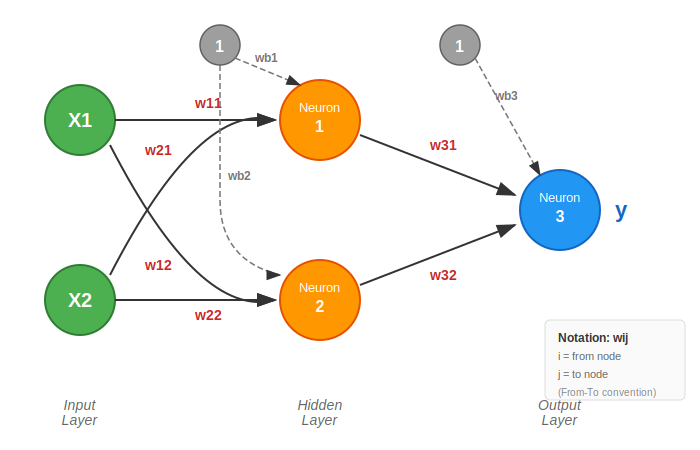
\includegraphics[width=0.6\textwidth]{images/network_architecture.jpeg}
\caption{2-2-1 神經網路架構}
\end{figure}

%-----------------------------------------------------------------------------
\subsection{PSO 訓練}
%-----------------------------------------------------------------------------

\subsubsection{適應度函數}

PSO 以損失函數值作為適應度評估,適應度函數為所有 4 個 XOR 訓練樣本的平均 MSE 損失:
\begin{equation}
\text{Fitness} = \frac{1}{4} \sum_{i=1}^{4} \frac{1}{2}(y_{\text{desired},i} - y_i)^2
\end{equation}
適應度越低表示該粒子(權重組合)的解越佳。

\subsubsection{參數設定}

使用 Clerc \& Kennedy 收斂係數:

\begin{table}[H]
\centering
\begin{tabular}{lrl}
\toprule
\textbf{參數} & \textbf{值} & \textbf{說明} \\
\midrule
粒子數量 & 1000 & num\_particles \\
慣性權重 $w$ & 0.729 & Inertia weight \\
認知係數 $c_1$ & 1.49445 & Cognitive coefficient \\
社會係數 $c_2$ & 1.49445 & Social coefficient \\
位置範圍 & $[-10, 10]$ & pos\_min, pos\_max \\
速度上限 & 4.0 & vel\_max \\
最大迭代 & 500 & max\_iter \\
目標損失 & 0.00001 & target\_loss \\
\bottomrule
\end{tabular}
\caption{PSO 參數設定}
\end{table}

\subsubsection{終止條件}

當滿足以下任一條件時停止搜尋:
\begin{enumerate}
    \item 達到最大迭代次數(500 次)
    \item 全域最佳損失值低於目標損失(0.00001)
\end{enumerate}

\subsubsection{粒子編碼}

每個粒子編碼為 9 維向量,對應網路的所有權重與偏置:
\begin{align*}
\text{Particle} = [&w_{11}^{(1)}, w_{12}^{(1)}, w_{21}^{(1)}, w_{22}^{(1)}, & \text{(隱藏層權重 4 個)} \\
                   &b_1^{(1)}, b_2^{(1)}, & \text{(隱藏層偏置 2 個)} \\
                   &w_1^{(2)}, w_2^{(2)}, & \text{(輸出層權重 2 個)} \\
                   &b^{(2)}] & \text{(輸出層偏置 1 個)}
\end{align*}

\subsubsection{速度與位置更新公式}

速度更新公式:
\begin{equation}
v_i^{t+1} = w \cdot v_i^t + c_1 r_1 (p_i - x_i^t) + c_2 r_2 (g - x_i^t)
\end{equation}

位置更新公式:
\begin{equation}
x_i^{t+1} = x_i^t + v_i^{t+1}
\end{equation}

其中 $p_i$ 為粒子個體最佳位置,$g$ 為全域最佳位置,$r_1, r_2 \in [0,1]$ 為隨機數。速度會被限制在 $[-v_{\max}, v_{\max}]$ 範圍內,位置會被限制在 $[\text{pos}_{\min}, \text{pos}_{\max}]$ 範圍內。

\subsubsection{最佳權重}

PSO 訓練後取得的最佳權重:

\begin{table}[H]
\centering
\begin{tabular}{lr}
\toprule
\textbf{權重/偏置} & \textbf{值} \\
\midrule
$w_{11}^{(1)}, w_{12}^{(1)}$ & 10.0, $-$10.0 \\
$w_{21}^{(1)}, w_{22}^{(1)}$ & $-$10.0, 10.0 \\
$b_1^{(1)}, b_2^{(1)}$ & 5.0068, 5.0068 \\
$w_1^{(2)}, w_2^{(2)}$ & $-$6.8010, $-$6.8010 \\
$b^{(2)}$ & 10.0 \\
\midrule
\textbf{Final Loss} & 0.00252 \\
\bottomrule
\end{tabular}
\caption{PSO 最佳權重}
\end{table}

\subsubsection{Loss 曲線}

\begin{figure}[H]
\centering
\includegraphics[width=0.85\textwidth]{images/xor_pso_loss.png}
\caption{XOR PSO 訓練 Loss 曲線}
\end{figure}

%-----------------------------------------------------------------------------
\subsection{Gradient Descent 訓練(比較)}
%-----------------------------------------------------------------------------

\subsubsection{參數設定}

\begin{table}[H]
\centering
\begin{tabular}{lrl}
\toprule
\textbf{參數} & \textbf{值} & \textbf{說明} \\
\midrule
學習率 & 3.0 & Learning rate \\
最大迭代 & 500 & max\_iter \\
目標損失 & 0.000001 & target\_loss \\
\bottomrule
\end{tabular}
\caption{SGD 參數設定}
\end{table}

\subsubsection{最佳權重}

\begin{table}[H]
\centering
\begin{tabular}{lr}
\toprule
\textbf{權重/偏置} & \textbf{值} \\
\midrule
$w_{11}^{(1)}, w_{12}^{(1)}$ & $-$5.790, 4.308 \\
$w_{21}^{(1)}, w_{22}^{(1)}$ & $-$5.783, 4.306 \\
$b_1^{(1)}, b_2^{(1)}$ & 2.181, $-$6.706 \\
$w_1^{(2)}, w_2^{(2)}$ & $-$8.440, $-$8.576 \\
$b^{(2)}$ & 4.187 \\
\midrule
\textbf{Final Loss} & 0.00257 \\
\bottomrule
\end{tabular}
\caption{SGD 最佳權重}
\end{table}

\subsubsection{Loss 曲線}

\begin{figure}[H]
\centering
\includegraphics[width=0.85\textwidth]{images/xor_sgd_loss.png}
\caption{XOR SGD 訓練 Loss 曲線}
\end{figure}

%-----------------------------------------------------------------------------
\subsection{測試結果}
%-----------------------------------------------------------------------------

使用 PSO 訓練的模型測試三組輸入:

\begin{table}[H]
\centering
\begin{tabular}{cc|c}
\toprule
$X_1$ & $X_2$ & 預測值 \\
\midrule
0.7 & 0.3 & 0.1442 \\
0.6 & 0.4 & 0.0364 \\
0.5 & 0.5 & 0.0290 \\
\bottomrule
\end{tabular}
\caption{PSO 模型測試結果}
\end{table}

\noindent \textbf{結果分析}:

三組測試輸入的預測值皆接近 0,這與直覺上「接近 (1,0) 的輸入應輸出接近 1」的預期不同。分析原因如下:

\begin{enumerate}
    \item \textbf{訓練資料特性}:XOR 只有 4 個精確的訓練點 (0,0), (0,1), (1,0), (1,1),神經網路學習到的決策邊界僅針對這些離散點最佳化。

    \item \textbf{決策邊界位置}:觀察 PSO 學到的權重,隱藏層的兩個神經元分別學習到 $X_1 - X_2$ 和 $X_2 - X_1$ 的特徵(權重為 $\pm 10$)。當 $X_1 \approx X_2$ 時(如 0.5, 0.5 或 0.6, 0.4),兩個隱藏神經元的輸出相近,導致最終輸出接近 0。

    \item \textbf{泛化行為}:這些測試點位於訓練資料的「中間區域」,神經網路將此區域歸類為接近 0 的輸出,這是該權重組合的自然泛化行為。
\end{enumerate}

若需要更符合「接近 (1,0) 則輸出接近 1」的行為,可考慮使用更多的訓練資料或調整網路架構。

%-----------------------------------------------------------------------------
\subsection{PSO vs Gradient Descent 比較}
%-----------------------------------------------------------------------------

\begin{table}[H]
\centering
\begin{tabular}{lcc}
\toprule
\textbf{指標} & \textbf{PSO} & \textbf{SGD} \\
\midrule
Final Loss & 0.00252 & 0.00257 \\
初始 Loss & 0.125 & 0.53 \\
收斂速度 & 極快(約 3-5 次迭代) & 較慢(約 200 次迭代) \\
計算成本 & 高(1000 粒子 × 500 次) & 低(單次梯度計算) \\
全域搜索 & 是 & 否(可能陷入局部最優) \\
\bottomrule
\end{tabular}
\caption{XOR 問題 PSO vs Gradient Descent 比較}
\end{table}

\textbf{結論}:對於 XOR 這種小規模、低維度問題,PSO 收斂速度遠優於 Gradient Descent,且最終 Loss 也略低。PSO 的全域搜索能力使其在前幾次迭代就能找到接近最優解的區域。

\newpage

%=============================================================================
\section{MNIST 手寫數字辨識}
%=============================================================================

\subsection{網路架構}

\begin{table}[H]
\centering
\begin{tabular}{ll}
\toprule
\textbf{項目} & \textbf{設定} \\
\midrule
架構 & 784-128-10 (MLP) \\
輸入層 & 784 節點 (28×28 灰階圖片) \\
隱藏層 & 128 節點 + ReLU Activation \\
輸出層 & 10 節點 + Softmax \\
損失函數 & Cross-Entropy \\
總參數量 & 101,770 \\
\bottomrule
\end{tabular}
\caption{MNIST 網路架構}
\end{table}

%-----------------------------------------------------------------------------
\subsection{PSO 訓練}
%-----------------------------------------------------------------------------

\begin{table}[H]
\centering
\begin{tabular}{lrl}
\toprule
\textbf{參數} & \textbf{值} & \textbf{說明} \\
\midrule
隱藏層大小 & 128 & hidden\_size \\
粒子數量 & 30 & num\_particles \\
慣性權重 $w$ & 0.729 & Inertia weight \\
$c_1, c_2$ & 1.49445 & Cognitive/Social \\
位置範圍 & $[-1, 1]$ & 較小範圍 \\
速度上限 & 0.5 & vel\_max \\
最大迭代 & 500 & max\_iter \\
批次大小 & 1000 & batch\_size \\
\bottomrule
\end{tabular}
\caption{MNIST PSO 參數設定}
\end{table}

\begin{figure}[H]
\centering
\begin{subfigure}{0.48\textwidth}
\includegraphics[width=\textwidth]{images/mnist_pso_loss.png}
\caption{Loss 曲線}
\end{subfigure}
\hfill
\begin{subfigure}{0.48\textwidth}
\includegraphics[width=\textwidth]{images/mnist_pso_accuracy.png}
\caption{Accuracy 曲線}
\end{subfigure}
\caption{MNIST PSO 訓練過程}
\end{figure}

\begin{figure}[H]
\centering
\includegraphics[width=0.7\textwidth]{images/mnist_pso_confusion.png}
\caption{MNIST PSO Confusion Matrix(Test Accuracy: $\sim$24\%)}
\end{figure}

%-----------------------------------------------------------------------------
\subsection{Gradient Descent 訓練}
%-----------------------------------------------------------------------------

\begin{table}[H]
\centering
\begin{tabular}{lrl}
\toprule
\textbf{參數} & \textbf{值} & \textbf{說明} \\
\midrule
隱藏層大小 & 128 & hidden\_size \\
學習率 & 0.1 & Learning rate \\
最大迭代 & 50 & max\_iter (epochs) \\
批次大小 & 64 & batch\_size \\
\bottomrule
\end{tabular}
\caption{MNIST SGD 參數設定}
\end{table}

\begin{figure}[H]
\centering
\begin{subfigure}{0.48\textwidth}
\includegraphics[width=\textwidth]{images/mnist_sgd_loss.png}
\caption{Loss 曲線}
\end{subfigure}
\hfill
\begin{subfigure}{0.48\textwidth}
\includegraphics[width=\textwidth]{images/mnist_sgd_accuracy.png}
\caption{Accuracy 曲線}
\end{subfigure}
\caption{MNIST SGD 訓練過程}
\end{figure}

\begin{figure}[H]
\centering
\includegraphics[width=0.7\textwidth]{images/mnist_sgd_confusion.png}
\caption{MNIST SGD Confusion Matrix(Test Accuracy: 95.9\%)}
\end{figure}

%-----------------------------------------------------------------------------
\subsection{PSO vs Gradient Descent 比較}
%-----------------------------------------------------------------------------

\begin{table}[H]
\centering
\begin{tabular}{lcc}
\toprule
\textbf{指標} & \textbf{PSO} & \textbf{SGD} \\
\midrule
Test Accuracy & $\sim$24\% & \textbf{95.9\%} \\
Final Loss & 4.06 & \textbf{0.033} \\
迭代次數 & 500 & 50 \\
總參數量 & 101,770 & 101,770 \\
\bottomrule
\end{tabular}
\caption{MNIST PSO vs Gradient Descent 比較}
\end{table}

\newpage
%-----------------------------------------------------------------------------
\subsection{分析與結論}
%-----------------------------------------------------------------------------

\textbf{為何 SGD 在 MNIST 上遠優於 PSO?}

\begin{enumerate}
    \item \textbf{維度詛咒}:MNIST 網路有 101,770 個參數。PSO 在如此高維空間中難以有效搜索,而 SGD 利用梯度資訊精確導航。

    \item \textbf{梯度資訊}:SGD 使用反向傳播計算梯度,每次更新都朝向損失降低的方向。PSO 僅依賴隨機搜索,缺乏方向性指引。

    \item \textbf{計算效率}:
    \begin{itemize}
        \item PSO:30 粒子 × 500 次迭代 = 15,000 次前向傳播(每粒子)
        \item SGD:60,000 訓練樣本 × 50 epochs / 64 batch = $\sim$47,000 次更新
        \item SGD 每次更新都利用梯度,資訊利用率遠高於 PSO
    \end{itemize}

    \item \textbf{收斂速度}:觀察 Loss 曲線,SGD 的 Loss 持續平穩下降,而 PSO 很快就停滯在局部區域。

    \item \textbf{粒子數量限制}:理論上增加粒子數可改善 PSO,但 101,770 維空間需要的粒子數量是天文數字,計算上不可行。
\end{enumerate}

\noindent \textbf{結論}:
\begin{itemize}
    \item 對於\textbf{低維}問題(如 XOR 的 9 個參數),PSO 是可行的替代方案
    \item 對於\textbf{高維}神經網路,Gradient Descent 類方法(SGD、Adam 等)是必要的選擇
    \item PSO 更適合用於\textbf{超參數最佳化}或\textbf{神經架構搜索}等離散/低維問題
\end{itemize}

\end{document}
